\documentclass[12pt,a4paper]{extarticle}
\usepackage{extsizes}
\usepackage{cmap} % для кодировки шрифтов в pdf
%\documentclass[a4paper,12pt]{article} %размер бумаги устанавливаем А4, шрифт 12пунктов
\usepackage[utf8]{inputenc}%включаем свою кодировку: koi8-r или utf8 в UNIX, cp1251 в Windows
\usepackage[T2A, T1]{fontenc}
\usepackage[english,russian]{babel}%используем русский и английский языки с переносами
\usepackage{amssymb,amsfonts,amsmath,mathtext,cite,enumerate,amsthm,mathenv} %подключаем нужные пакеты расширений
\numberwithin{equation}{section}
\usepackage{graphicx} %хотим вставлять в диплом рисунки?
\usepackage{indentfirst} % Красная строка
\graphicspath{{images/}}%путь к рисункам
\usepackage{hyperref}
\usepackage{framed}
\usepackage{color} %% это для отображения цвета в коде
\usepackage{listings} %% собственно, это и есть пакет listingsb
\usepackage{ucs}
\usepackage{latexsym}
\usepackage{bm}
\usepackage{array}
\usepackage{multirow}
\usepackage{ulem}
\usepackage{csvsimple}

\frenchspacing
%----------------ЗАГОЛОВКИ---------------------------
\usepackage{titlesec}

\titleformat{\chapter}[display]
    {\filcenter}
    {\MakeUppercase{\chaptertitlename} \thechapter}
    {8pt}
    {\bfseries}{}
 
\titleformat{\section}
    {\centering\normalsize\bfseries}
    {\thesection}
    {1em}{\MakeUppercase}
 
\titleformat{\subsection}
    {\normalsize\bfseries}
    {\thesubsection}
    {1em}{}

% Настройка вертикальных и горизонтальных отступов
%\titlespacing*{\chapter}{0pt}{-30pt}{8pt}
\titlespacing*{\section}{\parindent}{*4}{*4}
\titlespacing*{\subsection}{\parindent}{*4}{*4}
%------------------------------------------------------

%---------------------ПОЛЯ-----------------------------
\usepackage{geometry}
\geometry{left=3cm}
\geometry{right=1.5cm}
\geometry{top=2.4cm}
\geometry{bottom=2.4cm}


\makeatletter
\renewcommand{\@biblabel}[1]{#1.} % Заменяем библиографию с квадратных скобок на точку:
\makeatother

\makeatletter


\def\x@multispan#1{%
  \global\let\@tempa\@empty
  \@multicnt#1\relax
  \loop\ifnum\@multicnt>\@ne
  \xdef\@tempa{\@tempa\kern\dimen@i\hfill&\omit}%
   \advance\@multicnt\m@ne
  \repeat
  \@tempa\kern\dimen@i\hfill}


\long\def\xmulticolumn#1#2#3{%
 \omit
 \begingroup
   \def\@addamp{\if@firstamp \@firstampfalse \else
                \@preamerr 5\fi}%
  \@mkpream{#2}\@addtopreamble\@empty
  \endgroup
  \def\@sharp{#3}%
  \setbox\z@\hbox{{\@preamble}}%
\global\dimen@i\wd\z@
\global\divide\dimen@i#1\relax
 \ignorespaces
\x@multispan{#1}}
\makeatother

\linespread{1.3} % полуторный интервал
%\renewcommand{\baselinestretch}{1.5}
\renewcommand{\theenumi}{\arabic{enumi}}% Меняем везде перечисления на цифра.цифра
\renewcommand{\labelenumi}{\arabic{enumi}}% Меняем везде перечисления на цифра.цифра
\renewcommand{\theenumii}{.\arabic{enumii}}% Меняем везде перечисления на цифра.цифра
\renewcommand{\labelenumii}{\arabic{enumi}.\arabic{enumii}.}% Меняем везде перечисления на цифра.цифра
\renewcommand{\theenumiii}{.\arabic{enumiii}}% Меняем везде перечисления на цифра.цифра
\renewcommand{\labelenumiii}{\arabic{enumi}.\arabic{enumii}.\arabic{enumiii}.}% Меняем везде перечисления на цифра.цифра
%\renewcommand{\figurename}{Рисунок} 
\addto\captionsrussian{
\def\figurename{Рисунок}
\renewcommand{\refname}
    {Список использованных источников}
}
\usepackage[labelsep=space]{caption}
\DeclareCaptionLabelSeparator{bar}{ - }
\captionsetup{
  labelsep=bar
}

\usepackage{floatrow}
\DeclareFloatFont{tiny}{\tiny}
\floatsetup[table]{font=footnotesize,capposition=top}

%\usepackage{sectsty}

%\allsectionsfont{\centering}


\lstset{ %
language=Python,                 % выбор языка для подсветки (здесь это Python)
basicstyle=\scriptsize\sffamily, % размер и начертание шрифта для подсветки кода
numberstyle=\tiny,           % размер шрифта для номеров строк
stepnumber=1,                   % размер шага между двумя номерами строк
numbersep=5pt,                % как далеко отстоят номера строк от подсвечиваемого кода
backgroundcolor=\color{white}, % цвет фона подсветки - используем \usepackage{color}
showspaces=false,            % показывать или нет пробелы специальными отступами
showstringspaces=false,      % показывать или нет пробелы в строках
showtabs=false,             % показывать или нет табуляцию в строках
tabsize=2,                 % размер табуляции по умолчанию равен 2 пробелам
captionpos=t,              % позиция заголовка вверху [t] или внизу [b] 
breaklines=true,           % автоматически переносить строки (да\нет)
breakatwhitespace=false, % переносить строки только если есть пробел
escapeinside={\%*}{*)}   % если нужно добавить комментарии в коде
}

%\usepackage[explicit]{titlesec}
%\usepackage{textcase}
%\usepackage{microtype}
%\titleformat{\section}
  %{\normalfont\Large\scshape}{\large\thesection}{1em}{\textls{\MakeTextLowercase{#1}}}
\usepackage{tocloft}
\renewcommand{\cfttoctitlefont}{\hfil \normalfont\Large\bfseries\MakeUppercase}

\usepackage{inconsolata}
\newcommand{\norm}[1]{\left\lVert#1\right\rVert}%норма

\begin{document}
\begin{titlepage}
\begin{center}
\vspace{1.5em}
МИНИСТЕРСТВО ОБРАЗОВАНИЯ И НАУКИ РОССИЙСКОЙ ФЕДЕРАЦИИ\\
\vspace{\baselineskip}
ФЕДЕРАЛЬНОЕ ГОСУДАРСТВЕННОЕ АВТОНОМНОЕ\\
ОБРАЗОВАТЕЛЬНОЕ УЧРЕЖДЕНИЕ ВЫСШЕГО ОБРАЗОВАНИЯ\\
<<CАМАРСКИЙ ГОСУДАРСТВЕННЫЙ АЭРОКОСМИЧЕСКИЙ УНИВЕРСИТЕТ\\
ИМЕНИ АКАДЕМИКА С. П. КОРОЛЕВА>>
\vspace{\baselineskip}
\end{center}
{Институт (факультет) \uline{\hspace{5em}ракетно-космической техники\hfill}}\\
{Кафедра \uline{\hfillтеоретической механики\hfill}}\\
\vspace{32pt}
\begin{center}
ВЫПУСКНАЯ КВАЛИФИКАЦИОННАЯ РАБОТА\\
МАГИСТРА\\
\end{center}
\vspace{8pt}
\begin{center}
ПОЯСНИТЕЛЬНАЯ ЗАПИСКА\\
\end{center}
\begin{center}
\textbf{\uline{Удаление космического мусора путем электростатического взаимодействия}}
$\underset{\text{наименование темы}}{\textbf{\uline{с активным космическим аппаратом}}}$
\end{center}
\vspace{64pt}
Выпускник \uline{\hfill}$\underset{\text{(фамилия, имя, отчество)}}{\text{\uline{Асланов Евгений Владимирович}}}$\uline{\hfill}\\
Руководитель \uline{\hfill}($\underset{\text{(фамилия, И.О.)}}{\text{\uline{Асланов В.С.}}}$)\\
Рецензент \uline{\hfill}($\underset{\text{(фамилия, И.О.)}}{\text{\uline{Мантуров А.И.}}}$)\\
Нормоконтролёр \uline{\hfill}($\underset{\text{(фамилия, И.О.)}}{\text{\uline{Филиппова Т.С.}}}$)\\

\vspace{\fill}

\begin{center}
Самара 2017
\end{center}
\end{titlepage}
% это титульный лист
\setcounter{page}{2}
%\newpage
%\begin{figure}[H]
	\center{
\includegraphics[scale=0.5]{ssau_logo.png}}
\end{figure}
\begin{center}
\tiny{\textbf{МИНОБРНАУКИ РОССИИ\\
ФЕДЕРАЛЬНОЕ ГОСУДАРСТВЕННОЕ АВТОНОМНОЕ\\
ОБРАЗОВАТЕЛЬНОЕ УЧРЕЖДЕНИЕ ВЫСШЕГО ОБРАЗОВАНИЯ\\
<<CАМАРСКИЙ НАЦИОНАЛЬНЫЙ ИССЛЕДОВАТЕЛЬСКИЙ УНИВЕРСИТЕТ\\
ИМЕНИ АКАДЕМИКА С. П. КОРОЛЕВА>>\\}}
\end{center}
\begin{center}
  {Кафедра теоретической механики}
\end{center}
 \vspace{1.5em}
\begin{minipage}{0.5\linewidth}
  \begin{flushleft}
    \end{flushleft}
  \end{minipage}
  \begin{minipage}{0.5\linewidth}
  \begin{flushright}
  УТВЕРЖДАЮ\\
  Заведующий кафедрой\\
  \underline{\hspace{7em}}/Асланов В.С.\\
  <<\underline{\hspace{2em}}>> \underline{\hspace{7em}} 2017 г.\\
  \end{flushright}
 \end{minipage}
  \vspace{0.5em}
  
  \begin{center}
  	\textbf{Задание на выпускную квалификационную работу (ВКР)}
  \end{center}
  
  Студенту \uline{\hfill Асланову Евгению Владмировичу \hfill}группы \uline{1225М}
  \begin{enumerate}
  \item Тема работы \uline{Удаление космического мусора путем электростатического\hfill \break взаимодействия\hfill\break} утверждена приказом по университету от <<\uline{\hspace{2em}}>> \underline{\hspace{7em}} 2017 г. №\underline{\hspace{3em}}
  \item Исходные данные к работе: \uline{параметры пассивного и активного аппаратов:\hfill \break $\phi = 20000$В, $R_1 = 0.5$м, $R_{2a} = R_{2c} = 0.59$м, $R_{2b} = 0.65$м, $l = 1.5$м, $d = 15$м,\hfill \break $J = 1000$кг$\cdot$м${}^2$ \hfill ${}$}
  \item Перечень вопросов, подлежащих разработке в ВКР:
  \uline{1. Метод многих сфер для описания электростатического взаимодействия двух тел. 2.Моделирование\hfill \breakдвижения космического аппарата цилиндрической формы вокруг центра масс при электростатическом взаимодействии с активным спутником при постоянном расстоянии между их центрами масс с помощью метода многих сфер.\hfill \break3. Моделирование движения двух космических аппаратов как двух материальных точек при действии тяги на одном из них. 4. Моделирование движения пассивного космического аппарата цилиндрической формы с активным космическим\hfill \breakаппаратом.\hfill${}$}
  \item Дата выдачи задания: <<\underline{\hspace{2em}}>> \underline{\hspace{7em}} 2017 г.
  \item Срок предоставления на кафедру законченной ВКР: <<\underline{\hspace{2em}}>> \underline{\hspace{6em}} 2017 г.
  \end{enumerate}
\newpage
\noindentРуководитель ВКР\\
$\underset{\text{должность, степень}}{\text{\uline{Заведующий кафедрой, доктор технических наук}}}$
$\underset{\text{подпись}}{\text{\uline{\hspace{10em}}}}$
$\underset{\text{И.О.Фамилия}}{\text{\uline{/В.С. Асланов/}}}$\\
Задание принял к исполнению
$\underset{\text{подпись студента}}{\text{\uline{\hspace{17em}}}}$
$\underset{\text{И.О.Фамилия студента}}{\text{\uline{/\hspace{1em}Е.В. Асланов\hspace{1em}/}}}$
%\newpage
%\section*{Реферат}
\textbf{Выпускная квалификационная работа магистра}: 48 страниц, 40 рисунков, 4 источника, 3 приложения. 

\textbf{Презентация}: 24 слайда PDF.

\hspace{1pt}

ДИФФЕРЕНЦИАЛЬНОЕ УРАВНЕНИЕ ДВИЖЕНИЯ, УРАВНЕНИЕ ЛАГРАНЖА ВТОРОГО РОДА, КУЛОНОВСКОЕ ВЗАИМОДЕЙСТВИЕ, МЕТОД МНОГИХ СФЕР, УПРАВЛЕНИЕ ДВИЖЕНИЕМ

\hspace{1pt}

В работе рассматривается движение системы, состоящей из пассивного космического аппарата (верхней ступени ракеты) и активного космического аппарата, при кулоновском взаимодействии между объектами системы.
Такая связка может быть применена для бесконтактной уборки космического мусора.

Цель работы – исследовать применение метода многих сфер  для бесконтактного увода с орбиты космического мусора.
Также показать целесообразность применения метода многих сфер вместо постоянных зарядов при моделировании движения относительно центра масс и рассмотреть управление для такой модели.

С использованием метода многих сфер и уравнения Лагранжа второго рода было проведено моделирование для трёх случаев взаимодействия аппаратов:
\begin{itemize}
	\item При моделировании движения космического аппарата цилиндрической формы вокруг центра масс с активным спутником при поддержании постоянного расстояния между центрами масс двух космических аппаратов методом многих сфер,
	\item При моделировании движения двух космических аппаратов как двух материальных точек при действии тяги на одном из них,
	\item При моделировании движения пассивного космического аппарата цилиндрической формы и активного космического аппарата методом многих сфер.
\end{itemize}
При помощи системы Wolfram Mathematica произведено численное моделирование, решены системы уравнений для рассматриваемых систем и графически приведены результаты моделирования.
%\newpage
\tableofcontents % это оглавление, которое генерируется автоматически
%\newpage
%\section*{ВВЕДЕНИЕ}
\addcontentsline{toc}{section}{Введение}

На данный момент проблема уборки космического мусора встает всё острее, так как число закончивших свои программы спутников и ступеней ракет только увеличивается.
Так же, постоянно увеличивается число объектов, считающихся космическим мусором, за счет столкновений уже ставших мусором объектов.
Всё это выводит из оборота множество орбит.

Большинство контактных способов уборки мусора либо потенциально порождают новый мусор (гарпуны, взрывы), либо слишком сложны в управлении (сети).
Один из бесконтактных способов, находящийся в разработке, будет рассмотрен в этой работе.

В работе рассматривается движение вокруг центра масс пассивного космического аппарата цилиндрической формы при постоянном расстоянии между центрами масс аппаратов. Моделирование проводится с помощью метода многих сфер.
Так же будет рассмотрено моделирование взаимодействия космических аппаратов, представленных материальными точками, с приложением тяги к активному аппарату. 
Будут составлены и проанализированы тяги управления.
Будут рассмотрены движение вокруг центра масс пассивного космического аппарата цилиндрической формы в системе с активным космическим аппаратом. Будет произведено исследование управляющей функции.
\newpage
\section{Метод многих сфер для описания электростатического взаимодействия двух тел}
\label{SEC:MSM}

Метод многих сфер предназначен для аппроксимации электростатического взаимодействия между проводящими объектами произвольных форм.
Космический аппарат или космический мусор моделируется набором сфер с фиксированными размерами и относительными положениями (рис.\ref{ris:sp_msm})\cite{msm}.
Внешняя сфера используется для разрешения сил и вращающих моментов на теле для определения оптимального решения параметров модели.
Предположим далее, что оптимальные относительные положения и размеры $n$ сфер в модели уже определены.
Получившийся набор сфер должен перемещаться и вращаться как изначальное тело.
Внешнюю сферу так же можно заменить другим объектом общей формы, описанным с помощью набора заряженных сфер.
Для каждого объекта нужно определить начало отсчета. Для аппарата на рисунке \ref{ris:sp_msm} это будет точка $O$. 

\begin{figure}[H]
	\center{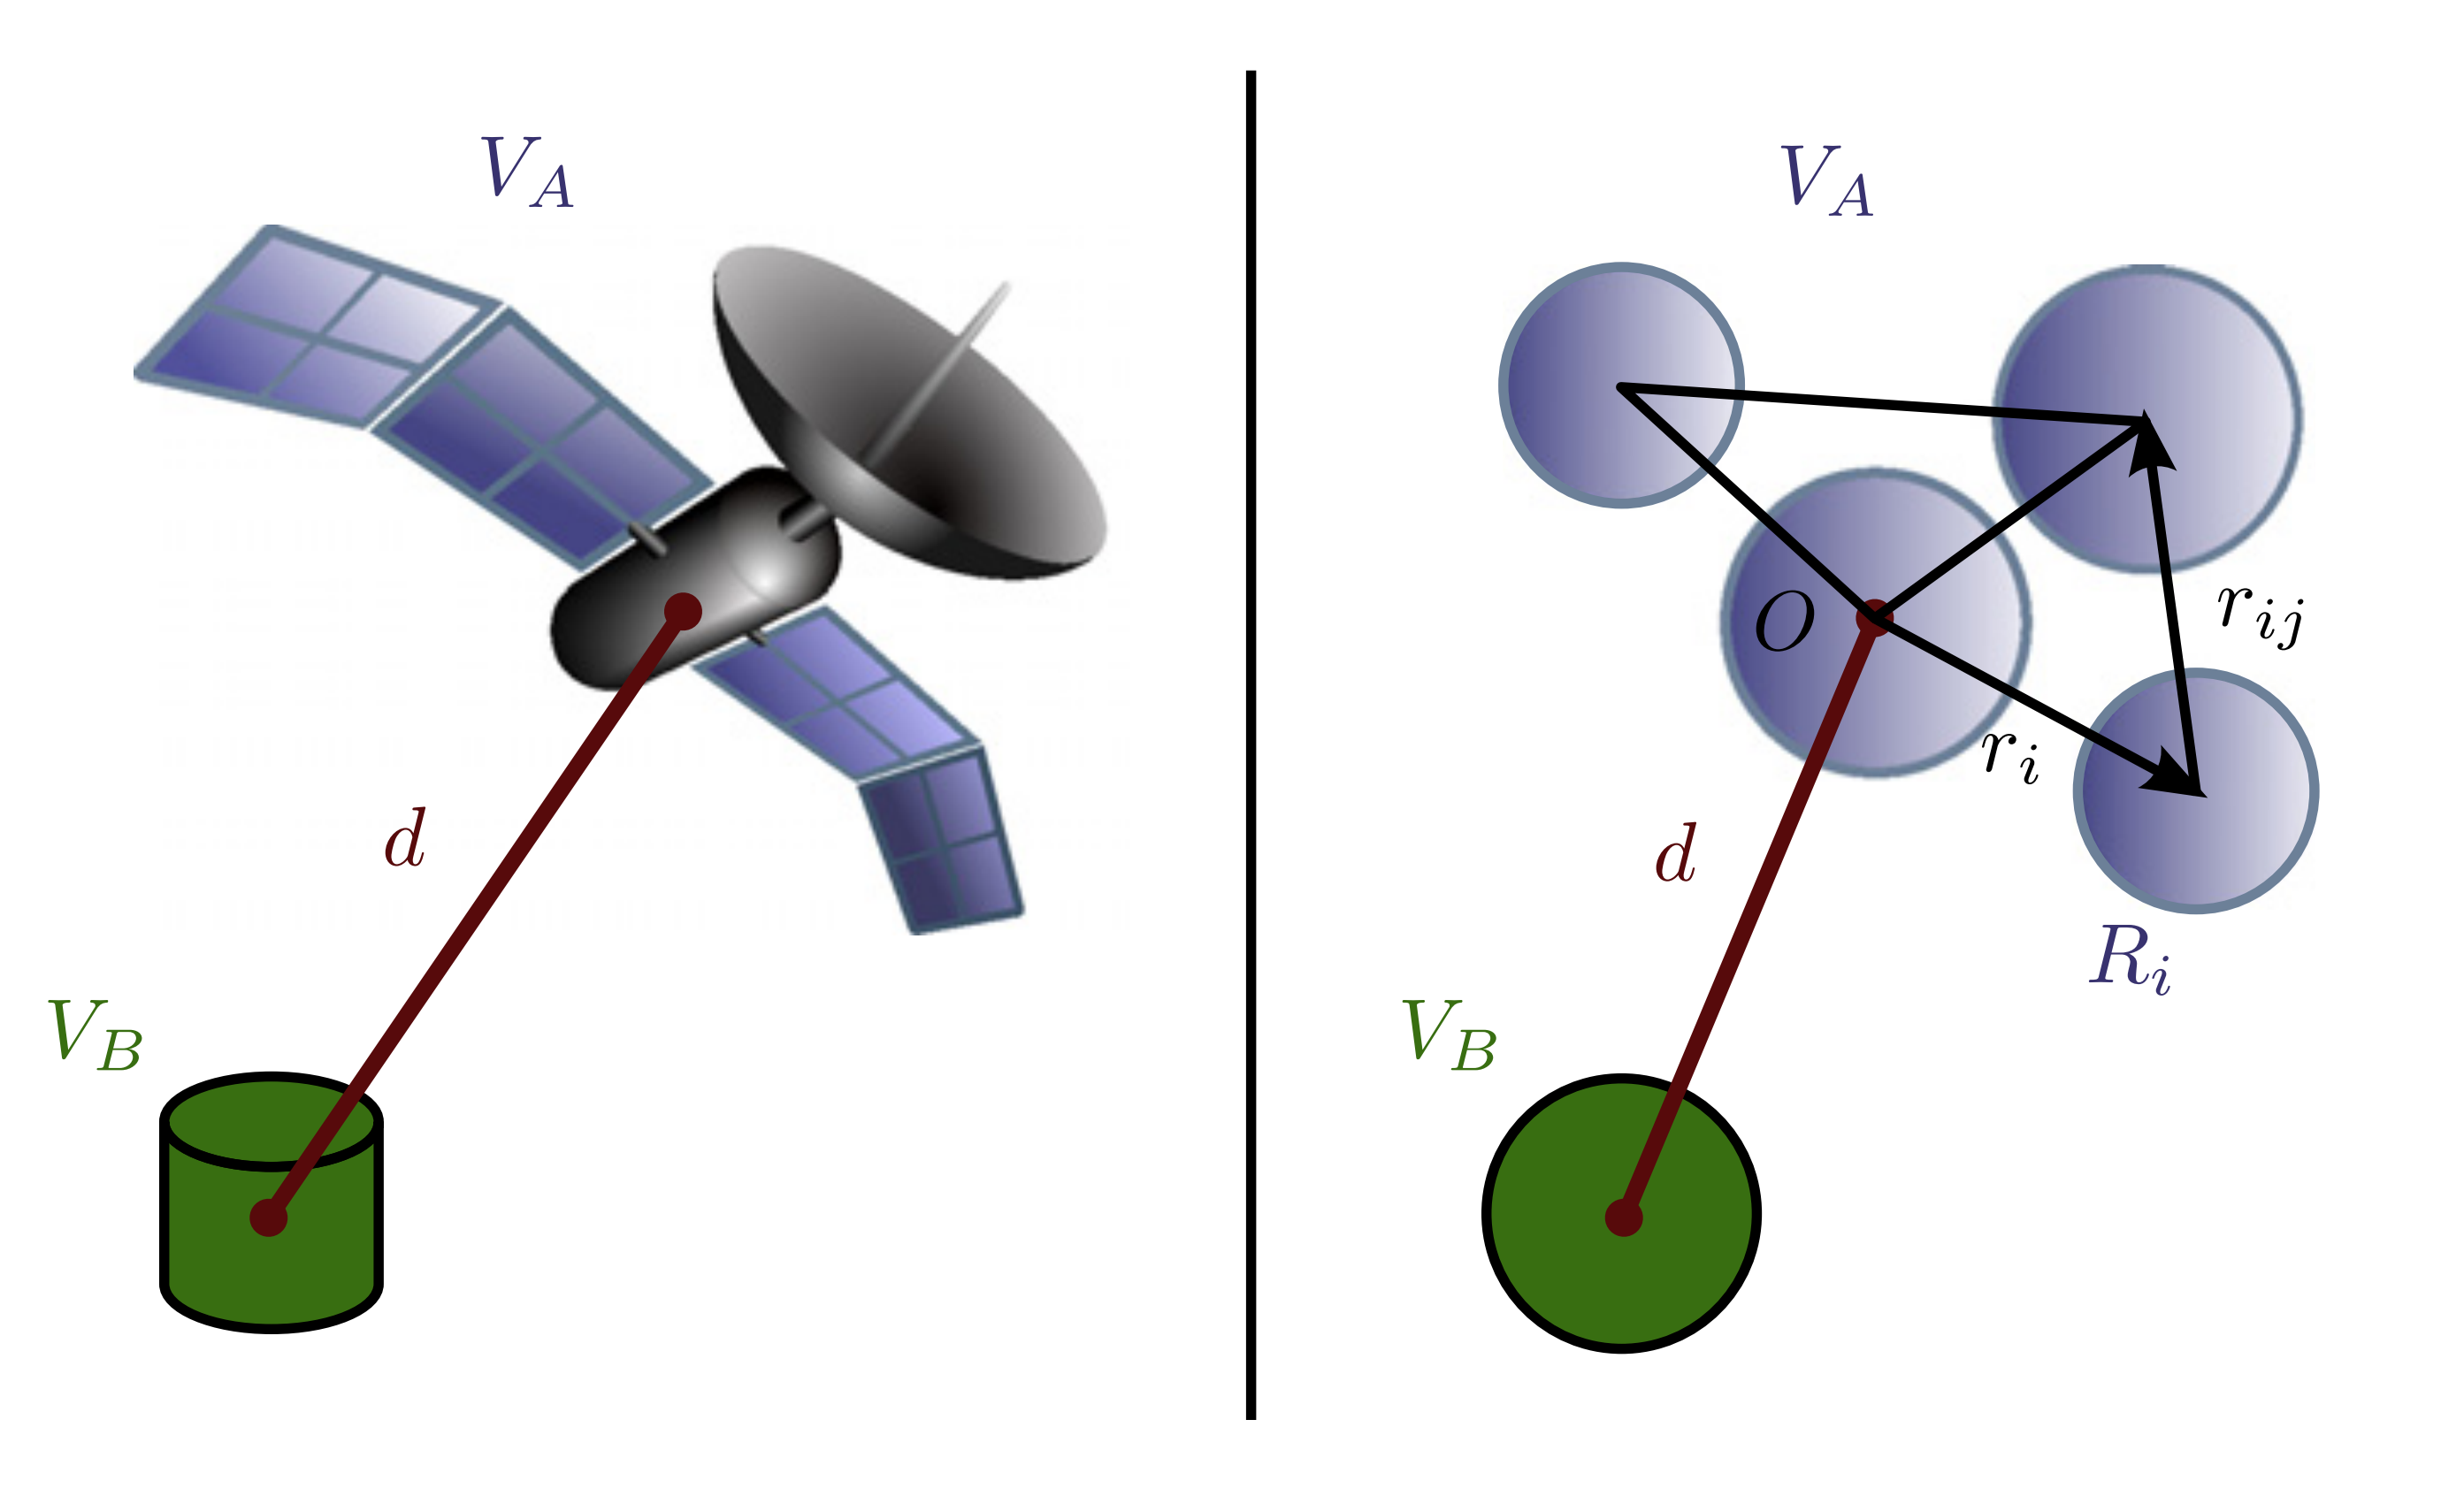
\includegraphics[scale=0.35]{spacecraft_msm.png}}
	\caption{Концептуальное описание метода многих сфер}
	\label{ris:sp_msm}
\end{figure}

Абсолютное электростатическое напряжение предполагается расположенным на космическом аппарате.
При этом кулоновская сила взаимодействия между сферами зависит от заряда каждой сферы.
Напряжение $\Phi_i$ на каждой сфере зависит как от заряда самой сферы, так и от заряда соседних с ней сфер и определяется по формуле \cite{2sph}:
\begin{equation}
\label{eq:voltage}
	\Phi_i = k_c \frac{q_i}{R_i} + \sum_{j=1,j\neq i}^{m} k_c \frac{q_j}{r_{i,j}},
\end{equation}
где $R_i$ – радиус $i$-ой сферы, $r_{i,j} = r_j - r_i$ – расстояние между центрами соседних сфер, $k_c = \frac{1}{4\pi\varepsilon_0} = 8.99 * 10^9 \frac{N*m^2}{C^2}$ – постоянная Кулона, $q_i$ – заряд $i$-ой сферы.

Линейные отношение из (\ref{eq:voltage}) для каждой из $m = n + 1$ сфер ($n$ сфер описывают тело и одна внешняя) в системе можно представить в матричном виде \cite{msm}:
\begin{equation}
\label{eq:voltage_matr}
	\vec{\Phi} = k_c [C_m]^{-1} \vec{q},
\end{equation}
где $\vec{\Phi} = [\Phi_A, \Phi_A, \dots, \Phi_A, \Phi_B]^T$ – вектор напряжений, $\vec{q} = [q_1, q_2, \dots, q_n, q_b]^T$ – вектор зарядов, $\Phi_A$ – напряжение каждой сферы тела, $\Phi_B$ – напряжение внешней сферы, $C_m$ – матрица ёмкостей, обратная матрица к которой имеет вид:
\begin{equation}
\label{eq:cm_inv}
	[C_m]^{-1} = 
	\begin{pmatrix}
		1/R_1	&	1/r_{1,2}	&	\dots		&	1/r_{1,n}	&	1/r_{1,B} \\
		1/r_{1,2}	&	1/R_1	&	\dots		&	\vdots		&	\vdots \\
		\vdots		&	\ddots		&	\ddots	&	\vdots		&	\vdots \\
		1/r_{n,1}	&	\dots			&	\dots		&	1/R_n	&	1/r_{n,B} \\
		1/r_{B,1}	&	\dots			&	\dots		&	1/r_{B,n}	&	1/R_B
	\end{pmatrix},
\end{equation}
где $\vec{r}_{i,B} = \vec{d} - \vec{r}_i$.

Далее, решив систему уравнений (\ref{eq:voltage_matr}) с помощью взятия обратной матрицы к (\ref{eq:cm_inv}), получим функции от времени для зарядов $q_i$.
Имея выражения для зарядов, можно вычислить силу взаимодействия сфер.
Тело предполагаем твёрдым, что дает нам постоянные положения сфер относительно друг друга.
Полная сила взаимодействия $F$ и вращающий момент $L_O$ для тела $A$ в точке $O$ описываются формулами (\ref{eq:force_msm}) и (\ref{eq:torque_msm}) соответственно \cite{msm}.

\begin{equation}
\label{eq:force_msm}
	\vec{F} = k_c q_B \sum_{i=1}^n \frac{q_i}{\norm{\vec{r}_{i,B}}^3}\vec{r}_{i,B}.
\end{equation}

\begin{equation}
\label{eq:torque_msm}
	\vec{L}_O = k_c q_B \sum_{i=1}^n \frac{q_i}{\norm{\vec{r}_{i,B}}^3} \vec{r}_i \times \vec{r}_{i,B}.
\end{equation}
\newpage
\section{Моделирование движения космического аппарата цилиндрической формы вокруг центра масс при электростатическом взаимодействии с активным спутником при постоянном расстоянии между их центрами масс с помощью метода многих сфер}
\label{SEC:3SPH}

Опишем конкретный случай моделирования с помощью метода многих сфер, описанного в разделе \ref{SEC:MSM}.
В качестве космического аппарата будем рассматривать цилиндрическое тело, которое будет представлять собой упрощенный вариант первой ступени ракеты.
Для перехода к электростатическому взаимодействию это тело заменим на три сферы.
Внешняя сфера описывает аппарат, производящий уборку космического мусора.
Для упрощения вычислений, расстояние между аппаратами $d$ будем считать постоянным.
Описанная схема представлена на рисунке \ref{ris:3sph}.

\begin{figure}[H]
	\center{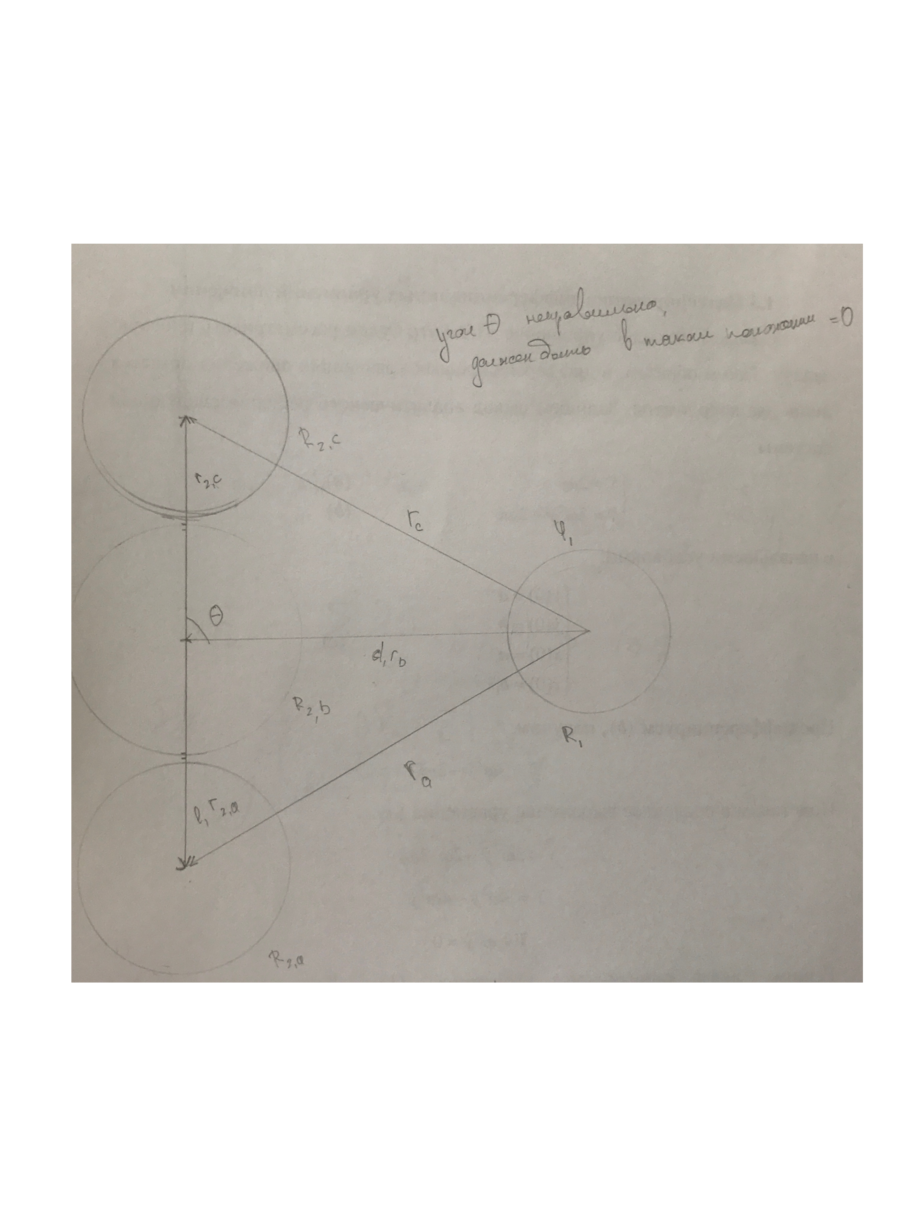
\includegraphics[scale=0.35]{3sph.png}}
	\caption{Замена космического аппарата сферами}
	\label{ris:3sph}
\end{figure}

Для моделирования взаимодействия составим обратную матрицу ёмкостей $[C_m]^{-1}$ (\ref{eq:cm_inv}):
\begin{equation}
\label{eq:3sph_cm}
	[C_m]^{-1} = 
	\begin{pmatrix}
		1/R_1	&	1/r_a	&	1/r_b	&	1/r_c\\
		1/r_a	&	1/R_{2a}	&	1/l		&	1/2l\\
		1/r_b	&	1/l		&	1/R_{2b}	&	1/l\\
		1/r_c	&	1/2l		&	1/l		&	1/R_{2c}
	\end{pmatrix},
\end{equation}
где $R_1$ – радиус внешней сферы, $R_{2a}$ – радиус сферы $A$ тела $2$, $R_{2b}$ – радиус сферы $B$ тела $2$, $R_{2c}$ – радиус сферы $C$ тела $2$, $l$ – расстояние между центрами соседних сфер (сферы $A$ и сферы $B$, сферы $B$ и сферы $C$),

\noindent $r_a = \norm{\vec{R}_a}$ – расстояние между центром внешней сферы и центром сферы $A$ тела $2$, $r_b = \norm{\vec{R}_b}$ – расстояние между центром внешней сферы и центром сферы $B$ тела $2$, $r_c = \norm{\vec{R}_c}$ – расстояние между центром внешней сферы и центром сферы $C$ тела $2$.

Для описания векторов $\vec{R_a}$, $\vec{R_b}$, $\vec{R_c}$ введем вектор $\vec{A}$  описывающий расстояния между центром тела $2$ и центром внешней сферы:
\begin{equation}
\label{eq:3sph_A}
	\vec{A} =
	\begin{pmatrix}
		0\\
		-d
	\end{pmatrix}.
\end{equation}
Так же введем вектора $\vec{L}_1$ и $\vec{L}_2$, описывающие расстояния между центрами сфер $B$ и $C$ и сфер $A$ и $B$:
\begin{equation}
\label{eq:3sph_l1}
	\vec{L}_1 = -\vec{L}_2,
\end{equation}
\begin{equation}
\label{eq:3sph_l2}
	\vec{L}_2 = 
	\begin{pmatrix}
		l \cos \theta(t)\\
		l \sin \theta(t)
	\end{pmatrix}.
\end{equation}

Имея (\ref{eq:3sph_A}), (\ref{eq:3sph_l1}) и (\ref{eq:3sph_l2}) запишем векторов $\vec{R_a}$, $\vec{R_b}$, $\vec{R_c}$:
\begin{equation}
\label{eq:3sph_Ra}
	\vec{R}_a = \vec{L}_1 - \vec{A},
\end{equation}
\begin{equation}
\label{eq:3sph_Rb}
	\vec{R}_b = -\vec{A},
\end{equation}
\begin{equation}
\label{eq:3sph_Rc}
	\vec{R}_c = \vec{L}_2 - \vec{A}.
\end{equation}

Имея (\ref{eq:3sph_Ra}), (\ref{eq:3sph_Rb}) и (\ref{eq:3sph_Rc}) можно получить обратную матрицу к матрице $[C_m]^{-1}$ (\ref{eq:3sph_cm}), тем самым решив уравнение (\ref{eq:voltage_matr}) и получив заряды сфер:
\begin{equation}
\label{eq:3sph_q_eq}
	\begin{pmatrix}
		q_1\\
		q_{2a}\\
		q_{2b}\\
		q_{2c}
	\end{pmatrix}
	= k_c C_m 
	\begin{pmatrix}
		-\phi\\
		\phi\\
		\phi\\
		\phi
	\end{pmatrix},
\end{equation}
где $q_1$ – заряд внешней сферы, $q_{2a}$ – заряд сферы $A$ тела $2$, $q_{2b}$ – заряд сферы $B$ тела $2$, $q_{2c}$ – заряд сферы $C$ тела $2$, $\phi$ – абсолютное значение напряжения для любой из сфер (оно берется одинаковым). 

Для получения зависимости угла $\theta$ от времени необходимо составить уравнение Лагранжа второго рода\cite{markeev}:
\begin{equation}
\label{eq:3sph_lag}
	\frac{d}{dt}\frac{\partial T}{\partial \dot{q_j}} - \frac{\partial T}{\partial q_j} = Q_j,
\end{equation}
где $q_j$ – обобщенные координаты, в нашем случае это $\theta(t)$, $Q_j$ – обобщенная сила,$T$ – кинетическая энергия, для нашей системы записанная в выражении:
\begin{equation}
\label{eq:3sph_kin}
	T = \frac{J \left(\frac{d \theta (t)}{dt}\right)^2}{2},
\end{equation}
где $J$ – момент инерции.

Обобщенная сила для обобщенной координаты $\theta$ имеет вид:
\begin{equation}
\label{eq:3sph_Qj}
	Q_\theta = \frac{\partial \vec{r}_{ba}}{\partial \theta(t)} \cdot F_{2a} + \frac{\partial \vec{r}_{bc}}{\partial \theta(t)} \cdot F_{2c},
\end{equation}
где вектор $\vec{r}_{ba} = L_1$ – вектор между центрами сфер $A$ и $B$, $\vec{r}_{bc} = L_2$ – вектор между центрами сфер $B$ и $C$, $F_{2a}$ и $F_{2c}$ – силы электростатического взаимодействия в центре внешней сферы:
\begin{equation}
\label{eq:3sph_F2a}
	F_{2a} = - \frac{k_c q_1 q_{2a}}{r_a^3} \vec{R}_a,
\end{equation}
\begin{equation}
\label{eq:3sph_F2c}
	F_{2c} = - \frac{k_c q_1 q_{2c}}{r_c^3} \vec{R}_c.
\end{equation}

Числено решив (\ref{eq:3sph_lag}) с учетом (\ref{eq:3sph_kin}), (\ref{eq:3sph_Qj}), (\ref{eq:3sph_F2a}) и (\ref{eq:3sph_F2c}) получим зависимость $\theta$ от времени.

Изменение угла $\theta$ для значений параметров $\phi = 20000$В, $R_1 = 0.5$м, $R_{2a} = R_{2c} = 0.59$м, $R_{2b} = 0.65$м, $l = 1.5$м, $d = 15$м, $J = 1000$кг$\cdot$м${}^2$ \cite{3sph} и максимальным временем $100000$ секунд изображено на рисунке (\ref{ris:3sph_theta_no_fix}).
Начальные условия:
\begin{equation}
	\begin{cases}
		\theta(0) = 1,\\
		\theta'(0) = 0.
	\end{cases}
\end{equation}

Обозначим числители выражений (\ref{eq:3sph_F2a})-(\ref{eq:3sph_F2c}) $S_a = - k_c q_1 q_{2a}$ и $S_c = - k_c q_1 q_{2c}$ соответственно и назовем это перетеканием заряда (рис. \ref{ris:3sph_flow_no_fix}).

\begin{figure}[H]
	\center{\includegraphics[scale=0.7]{msm_theta_d=15_no_fix.png}}
	\caption{Угол $\theta$ для заданных параметров}
	\label{ris:3sph_theta_no_fix}
\end{figure}

\begin{figure}[H]
	\center{\includegraphics[scale=0.7]{msm_flow_d=15_no_fix.png}}
	\caption{Перетекание заряда для заданных параметров}
	\label{ris:3sph_flow_no_fix}
\end{figure}

На рисунке \ref{ris:3sph_flow_no_fix} видно, что величина изменение заряда порядка $10^{-4}$.
Попробуем заменить перетекание заряда в выражениях для сил на фиксированную величину, взятую в точках пересечения $S_a$ и $S_c$, которые соответствуют $\theta = 0$.
Проведем вычисления для разных расстояний $d$.

\begin{figure}[H]
	\center{\includegraphics[scale=0.7]{msm_theta_d=20.png}}
	\caption{Угол $\theta$ для $d=20$м и максимального времени $150000$ секунд}
	\label{ris:3sph_theta_d=20}
\end{figure}

\begin{figure}[H]
	\center{\includegraphics[scale=0.7]{msm_flow_d=20.png}}
	\caption{Перетекание заряда для $d=20$м и максимального времени $150000$ секунд}
	\label{ris:3sph_flow_d=20}
\end{figure}

\begin{figure}[H]
	\center{\includegraphics[scale=0.7]{msm_theta_d=15.png}}
	\caption{Угол $\theta$ для $d=15$м и максимального времени $100000$ секунд}
	\label{ris:3sph_theta_d=15}
\end{figure}

\begin{figure}[H]
	\center{\includegraphics[scale=0.7]{msm_flow_d=15.png}}
	\caption{Перетекание заряда для $d=15$м и максимального времени $100000$ секунд}
	\label{ris:3sph_flow_d=15}
\end{figure}

\begin{figure}[H]
	\center{\includegraphics[scale=0.7]{msm_theta_d=10.png}}
	\caption{Угол $\theta$ для $d=10$м и максимального времени $50000$ секунд}
	\label{ris:3sph_theta_d=10}
\end{figure}

\begin{figure}[H]
	\center{\includegraphics[scale=0.7]{msm_flow_d=10.png}}
	\caption{Перетекание заряда для $d=10$м и максимального времени $50000$ секунд}
	\label{ris:3sph_flow_d=10}
\end{figure}

\begin{figure}[H]
	\center{\includegraphics[scale=0.7]{msm_theta_d=5.png}}
	\caption{Угол $\theta$ для $d=5$м и максимального времени $16000$ секунд}
	\label{ris:3sph_theta_d=5}
\end{figure}

\begin{figure}[H]
	\center{\includegraphics[scale=0.7]{msm_flow_d=5.png}}
	\caption{Перетекание заряда для $d=5$м и максимального времени $16000$ секунд}
	\label{ris:3sph_flow_d=5}
\end{figure}

\begin{figure}[H]
	\center{\includegraphics[scale=0.7]{{msm_theta_d=2.5}.png}}
	\caption{Угол $\theta$ для $d=2.5$м и максимального времени $3800$ секунд}
	\label{ris:3sph_theta_d=2.5}
\end{figure}

\begin{figure}[H]
	\center{\includegraphics[scale=0.7]{{msm_flow_d=2.5}.png}}
	\caption{Перетекание заряда для $d=2.5$м и максимального времени $3800$ секунд}
	\label{ris:3sph_flow_d=2.5}
\end{figure}

\begin{figure}[H]
	\center{\includegraphics[scale=0.7]{{msm_theta_d=1.8}.png}}
	\caption{Угол $\theta$ для $d=1.8$м и максимального времени $1300$ секунд}
	\label{ris:3sph_theta_d=1.8}
\end{figure}

\begin{figure}[H]
	\center{\includegraphics[scale=0.7]{{msm_flow_d=1.8}.png}}
	\caption{Перетекание заряда для $d=1.8$м и максимального времени $1300$ секунд}
	\label{ris:3sph_flow_d=1.8}
\end{figure}

Как видно из рисунков \ref{ris:3sph_theta_d=20} - \ref{ris:3sph_flow_d=1.8} при уменьшении расстояния $d$ фиксированное перетекание заряда (а значит и произведение зарядов) становится всё менее точным.
Отсюда можно сделать вывод, что метод многих сфер есть смысл применять при  сравнительно небольших расстояниях между объектами.
%\newpage
%\section*{ЗАКЛЮЧЕНИЕ}
\addcontentsline{toc}{section}{Заключение}

В данной работе проведено исследования системы из активного и пассивного космического аппаратов.

В разделе \ref{SEC:3SPH} рассмотрено движение вокруг центра масс пассивного космического аппарата цилиндрической формы при постоянном расстоянии между центрами масс аппаратов. Моделирование проводилось с помощью метода многих сфер.

В разделе \ref{SEC:2SPH} проведено моделирование взаимодействия космических аппаратов, представленных материальными точками, с приложением тяги к активному аппарату. Были составлены и проанализированы тяги управления.

В разделе \ref{SEC:2SPH_MSM} рассмотрено движение вокруг центра масс пассивного космического аппарата цилиндрической формы в системе с активным космическим аппаратом. Было произведено исследование управляющей функции. Моделирование так же проводилось с помощью метода многих сфер. Так как моделирование производилось в бессиловом поле, полученная модель пригодна для расчетов подобных взаимодействий на большом удалении от притягивающего центра или в поле действия силы тяжести (моделирование на земле).

В приложениях приведены программы для среды Wofram Mathematica.
\newpage
\addcontentsline{toc}{section}{Список использованных источников\bibliographystyle{gost780s} }
\begin{thebibliography}{99}
\bibitem{2sph} Slisko, J., Brito-Orta, R.A. On approximate formulas for the electrostatic force between two conducting spheres. American Journal of Physics 66 (4), 352–355, 1998.
\bibitem{msm} Daan Stevenson and Hanspeter Schaub. Multi-sphere method for modeling electrostatic forces and torques. Advances in Space Research, 51(1):10–20, Jan. 2013.
\end{thebibliography}
%\newpage
%\section*{ПРИЛОЖЕНИЕ А\break Исходный текст программы для решения задачи из раздела 2}\addcontentsline{toc}{section}{Приложение А Исходный текст программы для решения\break задачи из раздела \ref{sec:3sph}}
\lstinputlisting{3spheres.txt}
\newpage
\end{document}